\textbf{الف}
\\
کلاس 0:
میانگین 
\begin{bmatrix}
    0 \\
    0
\end{bmatrix}
است.
کوواریانس
\begin{bmatrix}
    9.5  & 7.5 \\
    7.5  & 9.5
\end{bmatrix}
است.
$\mu_0$
برابر با
$\frac{1}{3}$
است.\\
کلاس 1:
میانگین 
\begin{bmatrix}
    0 \\
    0
\end{bmatrix}
است.
کوواریانس
\begin{bmatrix}
    17  & 0 \\
    0  & 2
\end{bmatrix}
است.
$\mu_1$
برابر با
$\frac{1}{3}$
است.\\
کلاس2:
میانگین 
\begin{bmatrix}
    3 \\
    3
\end{bmatrix}
است.
کوواریانس
$\begin{bmatrix}
    9.5  & 7.5 \\
    7.5  & 9.5
\end{bmatrix}$$
است.
$\mu_2$
برابر با
$\frac{1}{3}$
است.


\textbf{ب}

\begin{center}    
\makebox[6em][c]{
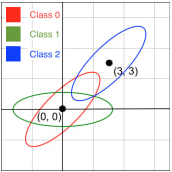
\includegraphics[height=7cm]{answers/contour.png}
}
\end{center}


\textbf{ج}
توابع
\lr{descriminant}
برای کلاس های 0 و 1 یک میانگین و یک ماتریس کوواریانس دارند در نتیجه هیچ
\lr{decision boundary}
ای برای این دو کلاس وجود نخواهد داشت.
\\
\\